\documentclass[letterpaper,10pt,draft]{book}
\usepackage[
  paper=letterpaper,
  lmargin=1in,
  rmargin=1in,
  tmargin=1in,
  bmargin=1in]{geometry}

%Uncomment below in the future to add indecies

% for adding index. Use \index{key} to put index keywords.
%\usepackage{multind}
%\makeindex{keyword}
%\makeindex{python}
%\makeindex{ui}

\newcommand{\mytitle}{\textbf{RGG User's Guide}}

% Make fancy headers and everything...
\usepackage{fancyhdr}
\pagestyle{fancy}
% Headers - left, center and right.
\lhead{}
\chead{\mytitle}
\rhead{}
% Footers - as before
%\lfoot{\scriptsize \emph{\svnInfoFile}}
\cfoot{\small \thepage}
%\rfoot{\scriptsize \emph{Rev: \svnInfoRevision , \svnInfoDate}}
\renewcommand{\headrulewidth}{0.5pt}
\renewcommand{\footrulewidth}{0.5pt}

%\addtolength{\headheight}{0.5pt} % make space for the rule
\setlength{\headheight}{14pt}
\fancypagestyle{plain}{%
  \fancyhead{} % get rid of headers on plain pages
  \renewcommand{\headrulewidth}{0pt} % and the line
}

% Now to define several macros for commonly used abbreviations and such
\usepackage{xspace}
\newcommand{\fixme}[1]{\footnote{{\color{red}#1}}}
\newcommand{\note}[1]{{\small\color{blue}[#1]}}
\newcommand{\todo}[1]{{\large\color{red}[TODO: #1]}}

\usepackage{url}
% Use in the form \url{http://mysite.co.uk/~marcus/} or \url!http://mysite.co.uk/~marcus/!

\usepackage[pdftex,final]{graphicx}
\usepackage[pdftex]{color}
\usepackage{setspace}

\usepackage{caption}
\usepackage{subcaption}

\usepackage{wrapfig}
\usepackage{float}


\usepackage{colortbl}
% 21st century - make some real links in the PDF, but keep the colors reasonable...
\usepackage[colorlinks=true,urlcolor=blue,citecolor=black,linkcolor=black,final=true]{hyperref}


\title{RGG User's Guide}
\author{Kitware, Inc.}

\begin{document}

\maketitle
\tableofcontents

\chapter{Introduction}
\label{chapter:Introduction}
Welcome to the Reactor Geometry Generator User's Guide.  Reactor Geometry Generator (RGG) is a program designed to aid you in modeling and meshing hexagonal and rectilinear reactor cores.  RGG uses Qt and VTK to produce an intuitive user interface.  By integrating a 3D view of the reactor with the meshing tools and combining them into one user interface, RGG streamlines the task of preparing a simulation mesh and enables real-time feedback that reduces accidental mistakes that waste hours of meshing.  RGG also interfaces with MeshKit tools to consolidate the meshing process, meaning that going from model to mesh is as easy as a button click.

This guide is designed to acquaint you with RGG's interface and to give you the knowledge and skills to pilot RGG successfully.  This book is organized in a concept/example manner, meaning that we cover concepts and the way that RGG thinks before we use those same ideas in an example.  Towards the end, we present a reference section that fully explains both the function of particular menus, buttons, and panes and what menu, button, or pane you must use to accomplish your objective.

\chapter{Main Application Components}
\label{chapter:Main Application Components}
Lorem ipsum dolor sit amet, consectetur adipiscing elit. Nunc eget ipsum aliquet, convallis eros ut, tempor velit. Phasellus ante erat, semper a lectus quis, consectetur dapibus lacus. Duis a justo ac nisl viverra tempus id ut justo. Curabitur sollicitudin pellentesque quam a sodales. Aenean iaculis nulla id sem pellentesque fermentum. Vestibulum ante ipsum primis in faucibus orci luctus et ultrices posuere cubilia Curae; Etiam felis nisi, placerat sed congue id, sodales id ligula. Nulla facilisi. Quisque est dui, laoreet vitae purus in, pellentesque dignissim mauris. Cras eu consectetur mauris.

\subsection{Main Window}
Vestibulum quis sagittis velit. Donec nec accumsan nibh, non consequat libero. Sed vulputate metus non leo aliquet scelerisque. Ut sed ullamcorper purus. Vestibulum lacus turpis, dignissim nec rhoncus quis, pellentesque scelerisque eros. Cras a pretium lectus. Aliquam at arcu lacinia, imperdiet nisi vel, pellentesque magna. Donec suscipit vestibulum nibh, vel adipiscing urna posuere ac.

\subsection{Material/Model Panel}
Etiam ut volutpat eros. Lorem ipsum dolor sit amet, consectetur adipiscing elit. Nulla convallis vulputate massa ac varius. Morbi varius felis non magna rhoncus, ac venenatis dui blandit. Mauris eu vestibulum augue. Morbi nec nibh urna. Quisque accumsan eros sed est rhoncus lacinia. In hac habitasse platea dictumst. Cras ullamcorper metus at massa dignissim viverra. Sed ullamcorper urna nunc, in tincidunt eros pharetra sed. Etiam consequat diam consequat, pharetra neque facilisis, pellentesque elit.

\subsection{Task Panel}
Etiam hendrerit, sapien ac euismod tincidunt, nulla dolor hendrerit sapien, nec blandit velit metus eu nisi. Nunc tempus, quam eu ultrices dapibus, sapien est vehicula arcu, a ornare neque leo vitae lacus. Interdum et malesuada fames ac ante ipsum primis in faucibus. Praesent blandit urna ut pretium scelerisque. Sed lobortis diam et dolor posuere, sed molestie mi condimentum. Mauris feugiat arcu ligula, eget convallis ipsum mollis sed. In a porttitor arcu. Suspendisse gravida adipiscing arcu. Integer pretium odio magna, id dapibus libero mollis eget. Donec nec diam ipsum.

\subsection{Reactor Core View}
Ut tincidunt, velit eget aliquam tincidunt, odio odio facilisis massa, viverra vulputate mi tortor et risus. Morbi cursus sit amet nisl vel cursus. Vivamus lobortis porta aliquam. Quisque non consequat velit. Class aptent taciti sociosqu ad litora torquent per conubia nostra, per inceptos himenaeos. Cras ut ante massa. Nullam ac felis ac elit vestibulum egestas. Donec molestie magna eget massa iaculis tincidunt. Nullam sed tristique ante, ac aliquet quam. Etiam quis placerat ipsum, ornare eleifend dolor. Pellentesque sed nisl aliquet, dignissim sapien in, sodales eros. Duis sollicitudin mi sed consectetur pellentesque.

\subsection{Assembly View}
Nam auctor condimentum nisi in aliquet. Suspendisse potenti. Nunc bibendum, risus ac fermentum venenatis, nisi ipsum interdum nibh, eu elementum orci ipsum ac felis. Integer congue tristique iaculis. Nam ipsum tortor, sodales fermentum tincidunt ut, iaculis eu dui. Duis interdum nibh at mauris vehicula commodo. Quisque congue aliquet sagittis. Ut at nisl turpis. Donec non velit et purus blandit consequat vel ut quam. Nulla ut tortor mattis, volutpat est at, iaculis velit. Ut tristique neque et dui tristique ultrices. Sed id aliquam dui. Sed imperdiet vitae lorem sit amet egestas. Proin odio ante, dignissim vestibulum rutrum interdum, eleifend eu quam. 

\subsection{Duct View}
Nulla ac lectus in nisl elementum suscipit id ac eros. Donec vel ante odio. Donec orci leo, varius eu quam vitae, dapibus commodo lorem. Sed luctus, ante id sagittis sagittis, lorem risus convallis leo, eget fermentum nunc elit vitae nisi. Interdum et malesuada fames ac ante ipsum primis in faucibus. Aenean sed risus quam. Fusce consectetur sem mi, in laoreet mi cursus vel. Vivamus pharetra, ipsum auctor tristique blandit, ante augue dapibus mauris, vel fermentum nibh urna ut erat. Mauris dignissim, nulla vitae accumsan consequat, turpis felis bibendum orci, ac eleifend neque eros vitae dui. Pellentesque tincidunt vulputate lacus in convallis.

\subsection{Pin Editing}
Aliquam vitae vulputate odio. Fusce mollis scelerisque nunc sed tristique. Aliquam hendrerit egestas orci, nec ultrices justo mattis eget. Duis nunc augue, malesuada eget sollicitudin vitae, consectetur non urna. Nulla tincidunt sagittis malesuada. Ut eleifend, risus vel vulputate tincidunt, lacus diam facilisis mi, at aliquet metus libero a nibh. Etiam magna libero, bibendum at semper interdum, fermentum vitae ante. Vestibulum et eleifend lacus. Quisque adipiscing fermentum tellus. Donec blandit nec lectus non luctus. Donec et erat dictum, lobortis lacus quis, tincidunt massa. Nunc tempus sollicitudin tempor.

\chapter{Example -- Building a Rectangular Core}
\label{chapter:Example -- Building a Rectangular Core}
\subsection{Creating an Assembly Duct Composed of Water}

First, create a new rectilinear core, and add a new duct to the assembly by following ~\ref{fig:Rect1}.

\begin{figure}[htb]
\begin{center}
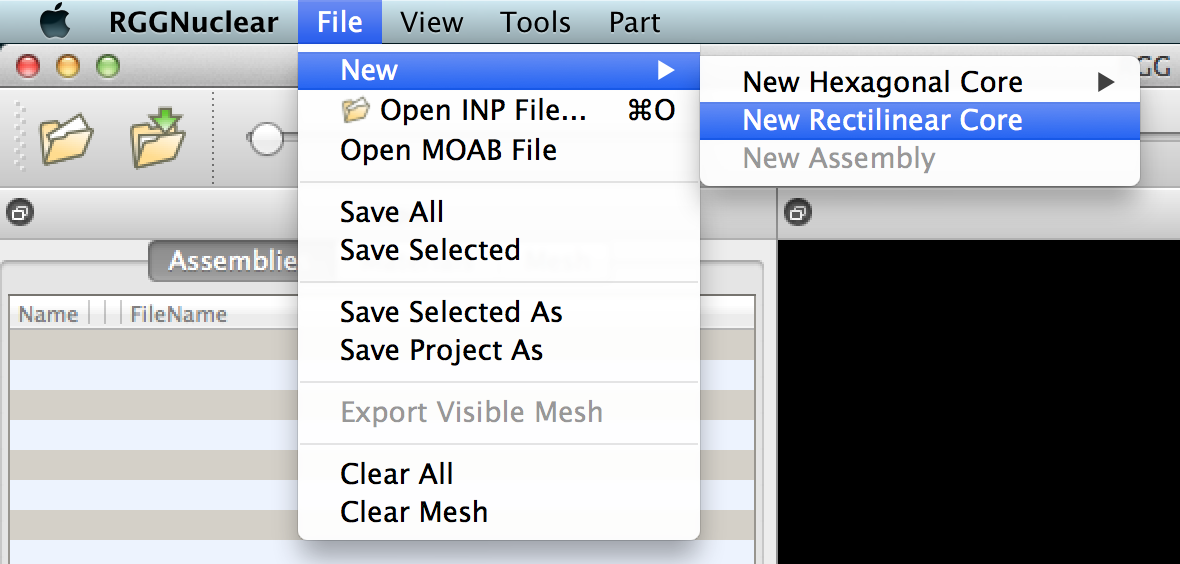
\includegraphics[width=0.5\linewidth]{Images/rect-1e1.png}
\caption{Select the option to create a new rectilinear assembly duct.}
\label{fig:Rect1}
\end{center}
\end{figure}

This results in a core with a single assembly with a duct of unknown material shown in ~\ref{fig:NewRect}.

\begin{figure}[htb]
\begin{center}
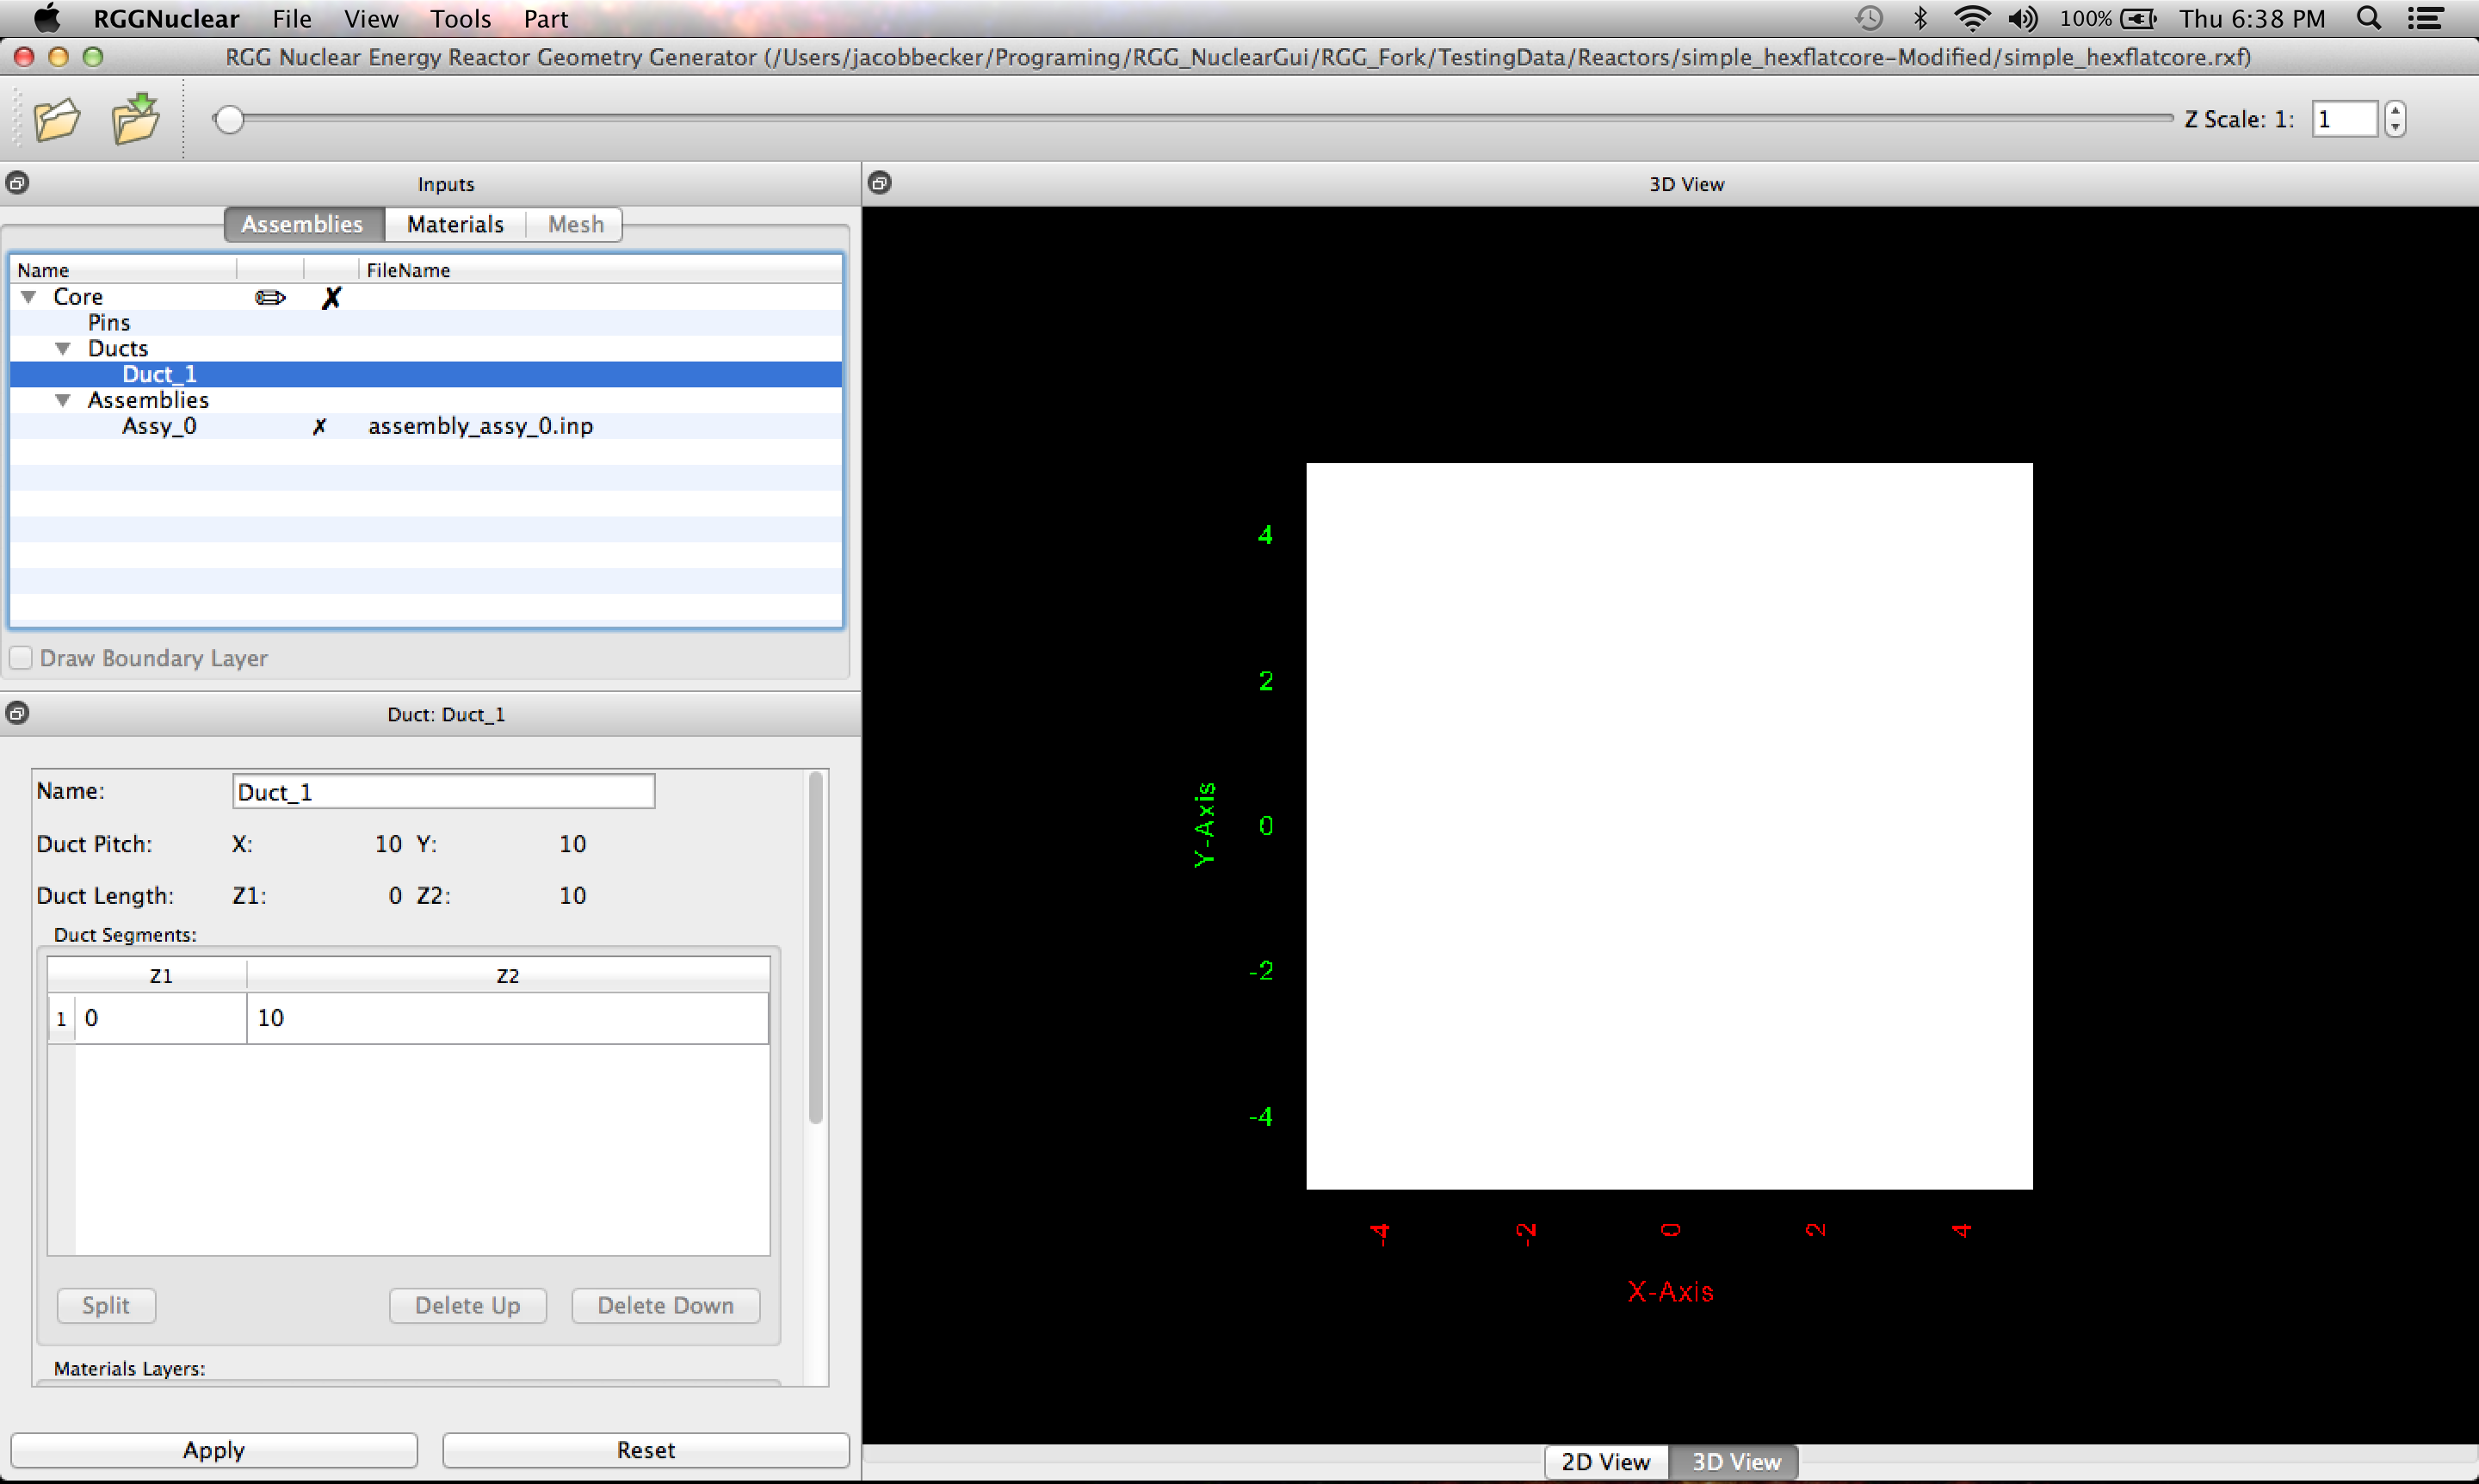
\includegraphics[width=0.5\linewidth]{Images/rect-init-model.png}
\caption{The initial rectangular core.}
\label{fig:NewRect}
\end{center}
\end{figure}

Now, to adjust the size of the duct, select the "Assembly Defaults" tab in Core's Properties Panel.  In this example, we are going to set the "Duct Thickness" to 15 (~\ref{fig:SetRectDuctDem}).

\begin{figure}[htb]
\begin{center}
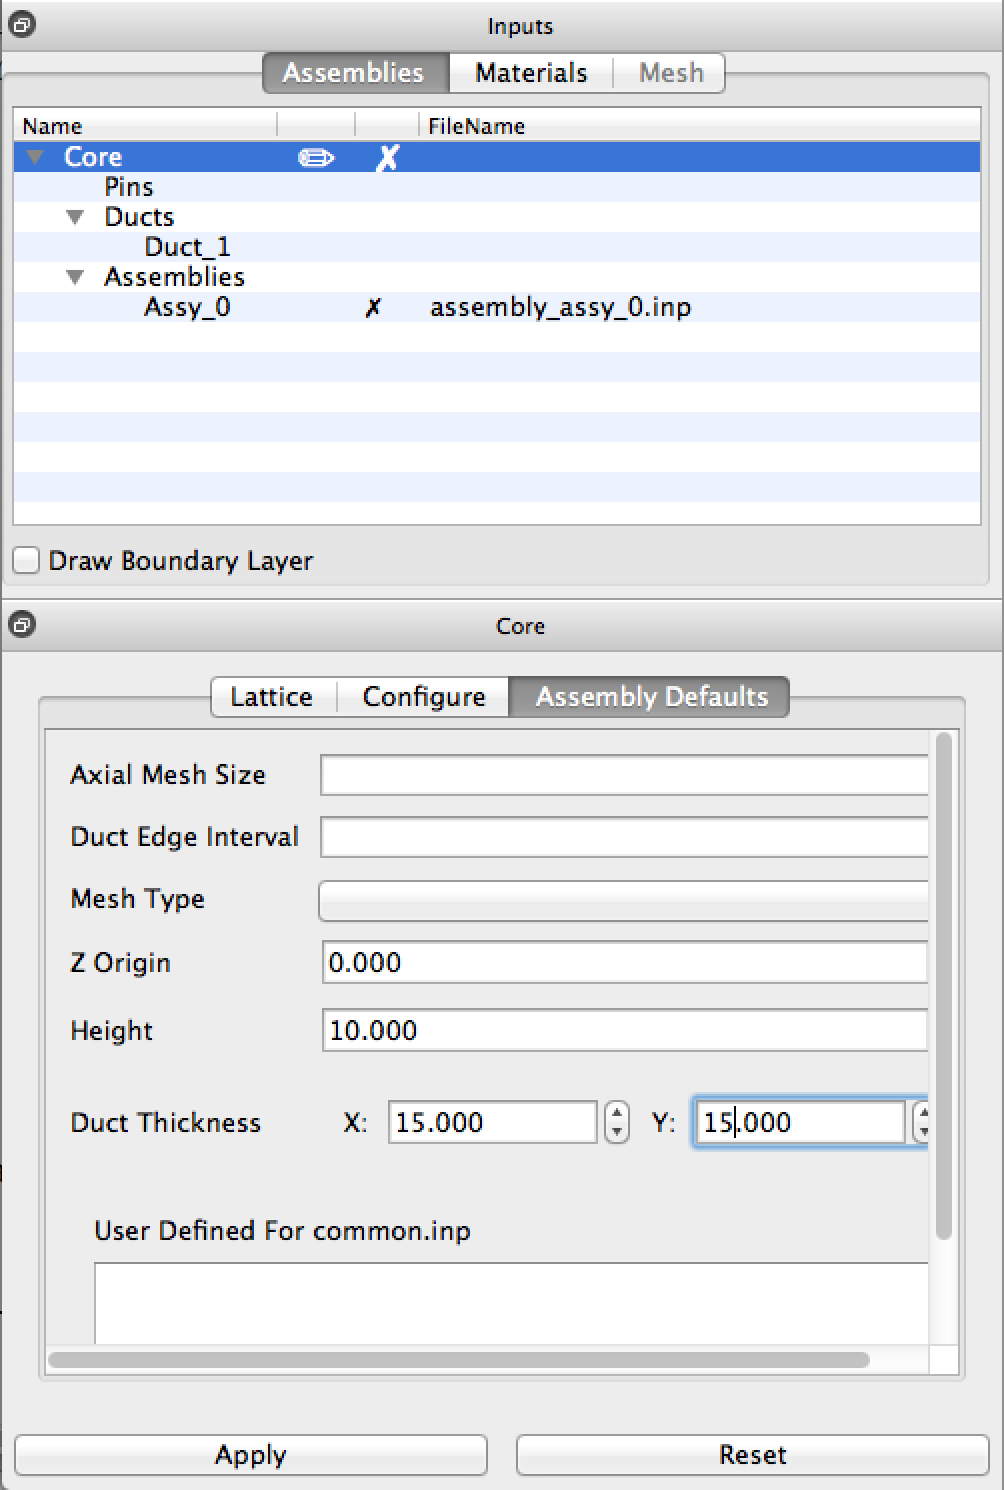
\includegraphics[width=0.5\linewidth]{Images/rect-set-dim.png}
\caption{The initial rectangular core.}
\label{fig:SetRectDuctDem}
\end{center}
\end{figure}

Next adjust the material of the Duct.  In the Inputs Panel, select the Duct.  Then, in the Duct's Properties Panel, select the first Duct Segment.  This populates Material Layers with the Duct Segments materials.  Now, select water in the material drop down box drop (~\ref{fig:rectSetMaterial}).  Then press Apply.  The result should look like ~\ref{fig:rectDuctResult}.

\begin{figure}
\centering
\begin{subfigure}{.5\textwidth}
  \centering
  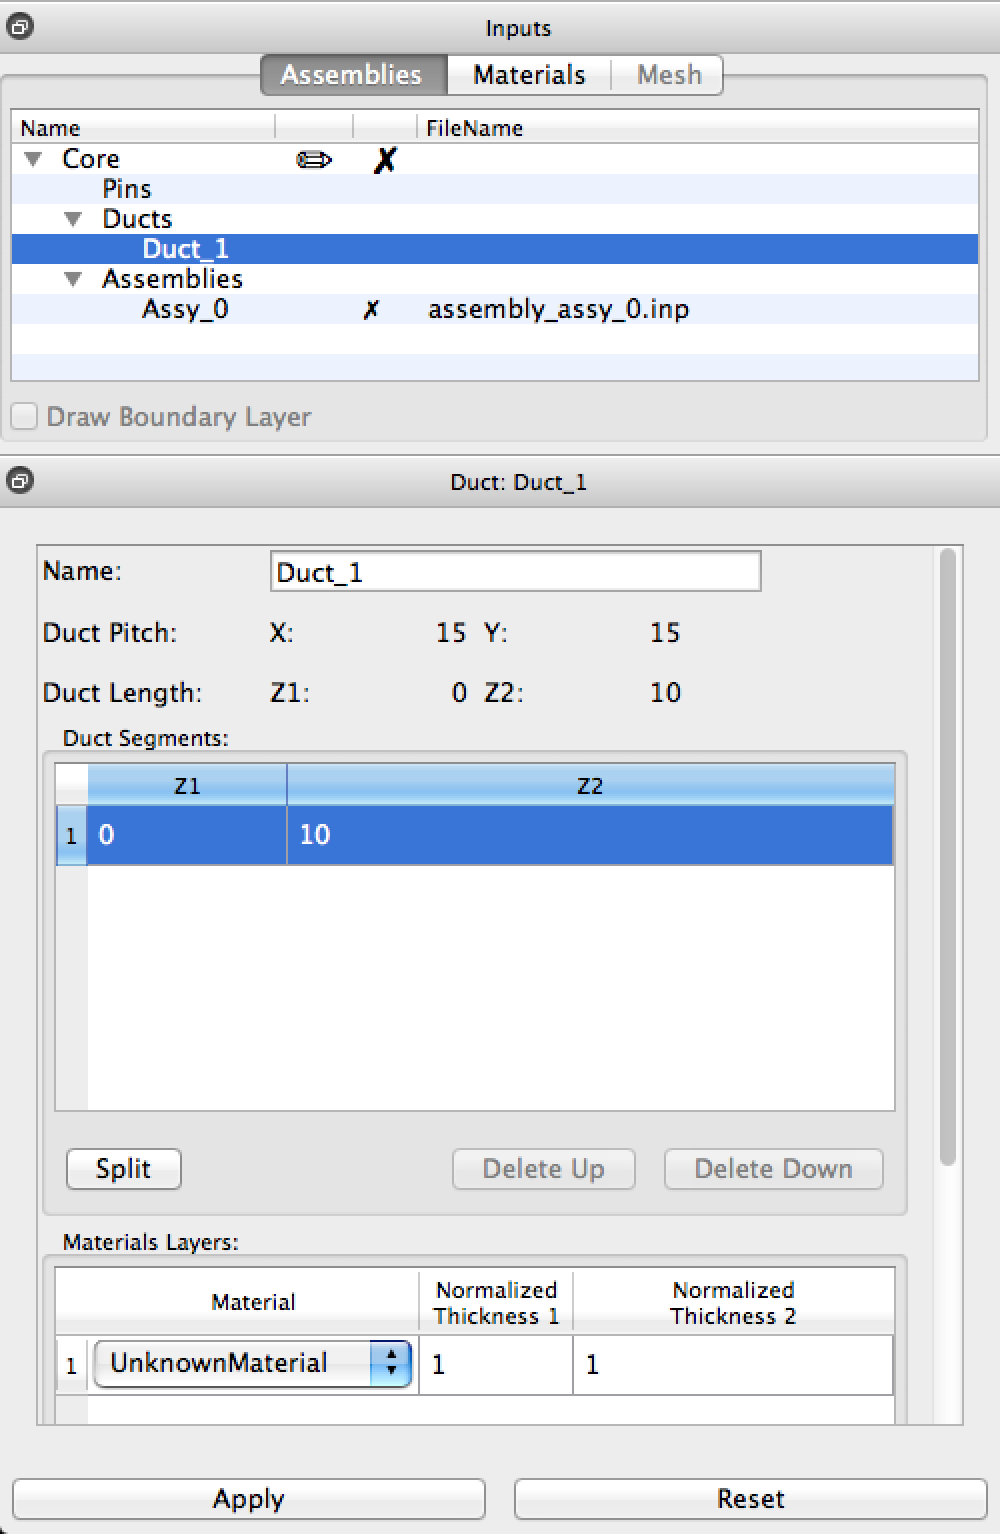
\includegraphics[width=0.7\linewidth]{Images/rect-set-material.png}
  \caption{Setting material of the duct.}
  \label{fig:rectSetMaterial}
\end{subfigure}%
\begin{subfigure}{.5\textwidth}
  \centering
  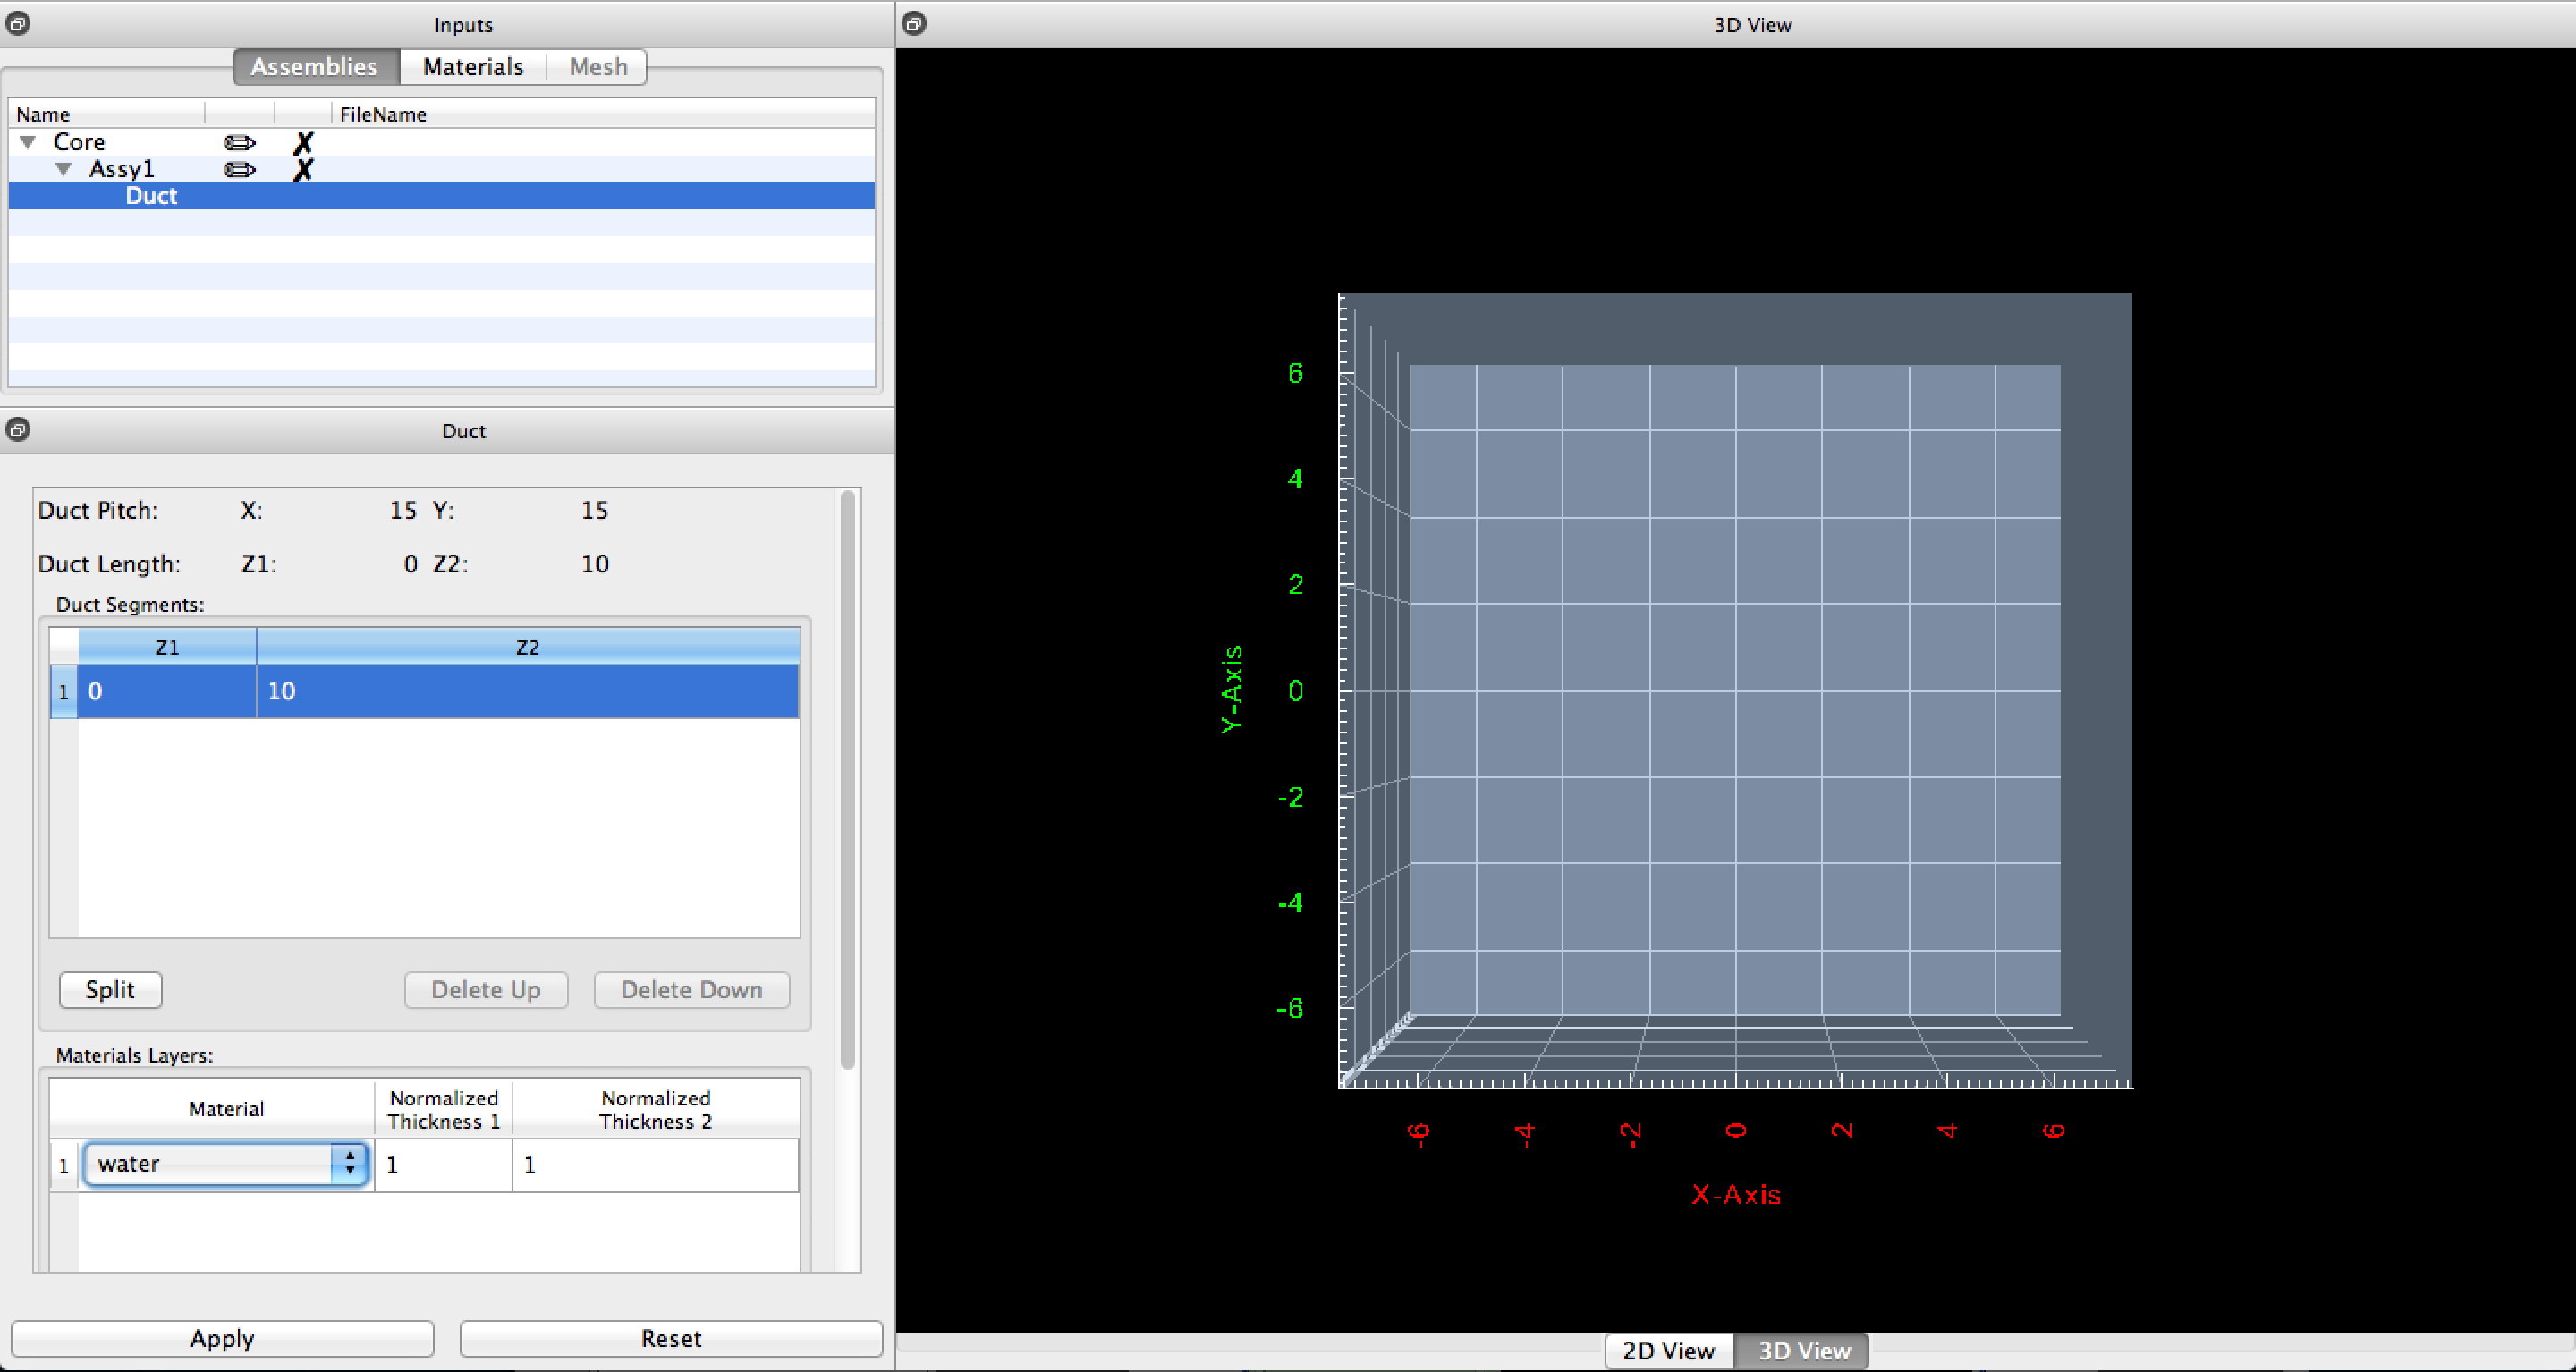
\includegraphics[width=0.9\linewidth]{Images/rect-duct-result.png}
  \caption{The final product.}
  \label{fig:rectDuctResult}
\end{subfigure}
\caption{Finished water duct.}
\label{fig:test}
\end{figure}

\clearpage

\subsection{Creating a Fuel Pin}

Right-click on the assembly and this time choose ``Create Pin''.

\subsubsection{Changing the Parameters}

Choose the dimensions of the pin to correspond to the dimensions of your duct.  In our case we have used a length of 4, corresponding to the height of the duct.

\begin{figure}[htb]
\begin{center}
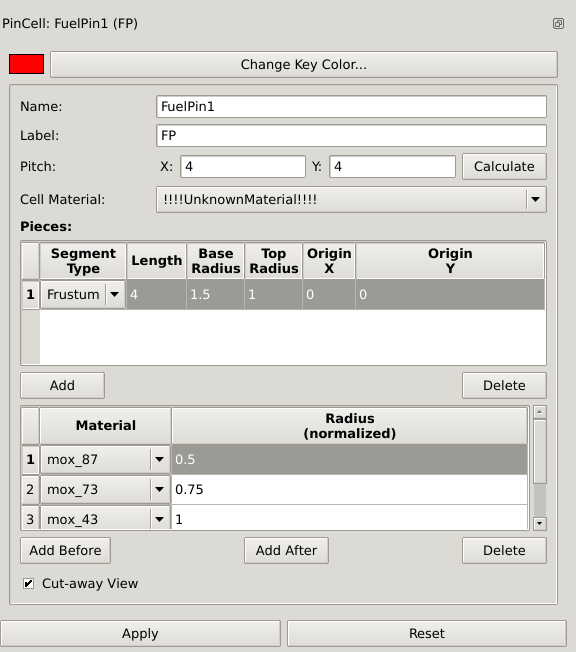
\includegraphics[width=0.4\linewidth]{Images/rect-5.png}
\caption{Fuel pin parameters.}
\label{fig:Rect5}
\end{center}
\end{figure}

Changing the key color and label is recommended, because later this will make the fuel pin more recognizeable while organizing the assembly.

\begin{wrapfigure}{r}{0.5\textwidth}
  \begin{center}
    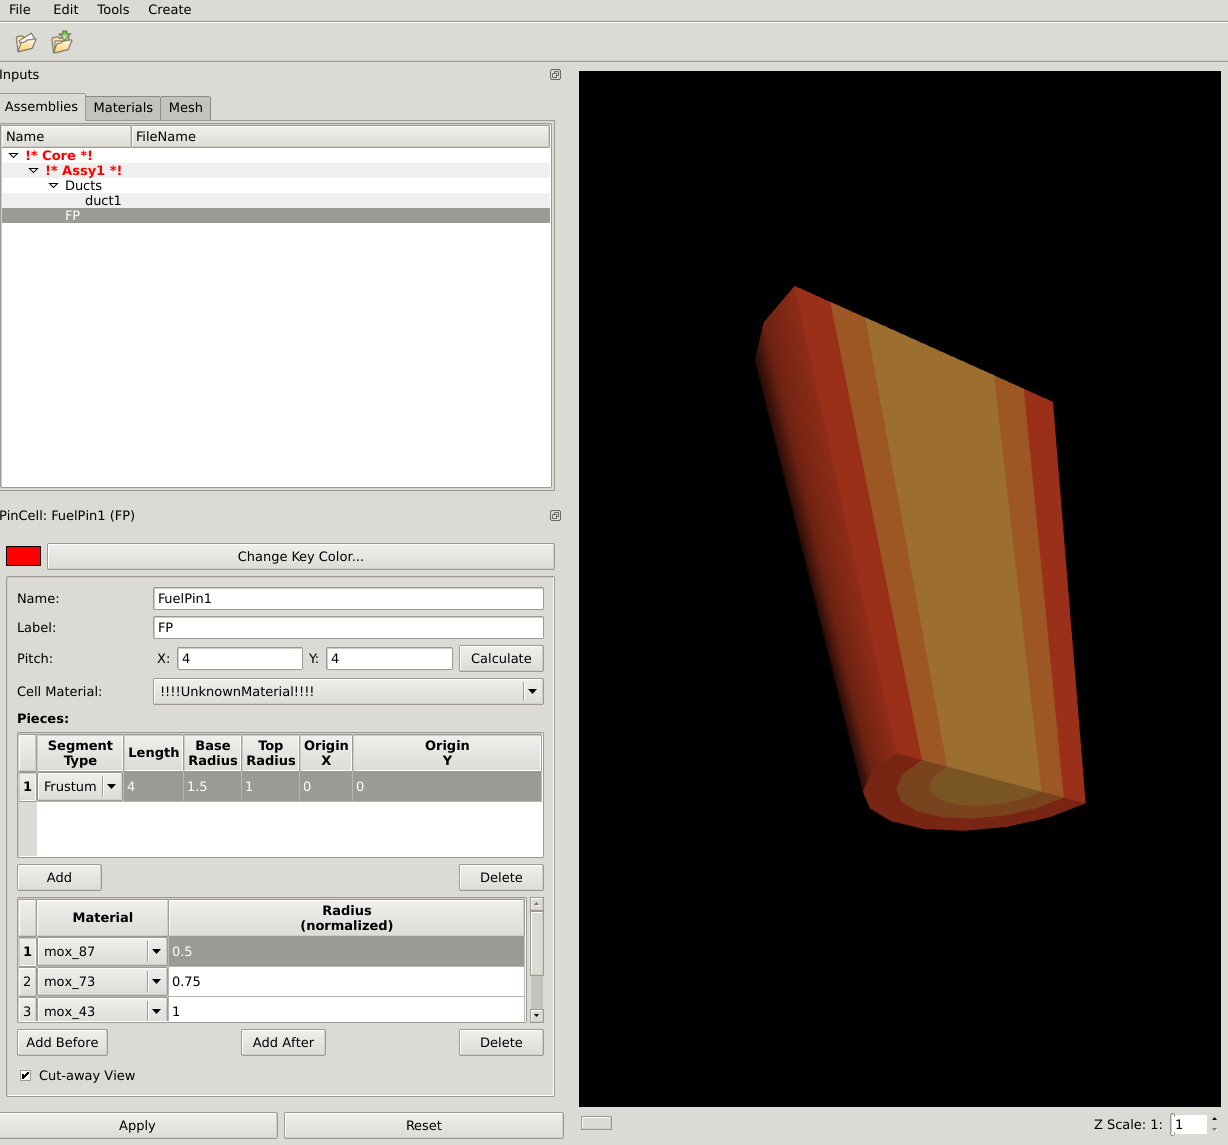
\includegraphics[width=0.48\textwidth]{Images/rect-6}
  \end{center}
  \caption{Final fuel pin product.}
  \label{fig:Rect6}
\end{wrapfigure}
Using the ``Add Before'' button, you can create a fuel pin with different layers of materials.  Refer to ~\ref{fig:Rect5} for the parameters used for our example, and ~\ref{fig:Rect6} to view the final product.

Note also the option to toggle the fuel pin's shape between a cylinder and a frustum.  The ``Cutaway view'' helps to view how the different materials are distributed within the fuel pin.

\subsection{Creating a Control Rod}
\begin{wrapfigure}{r}{0.5\textwidth}
  \begin{center}
    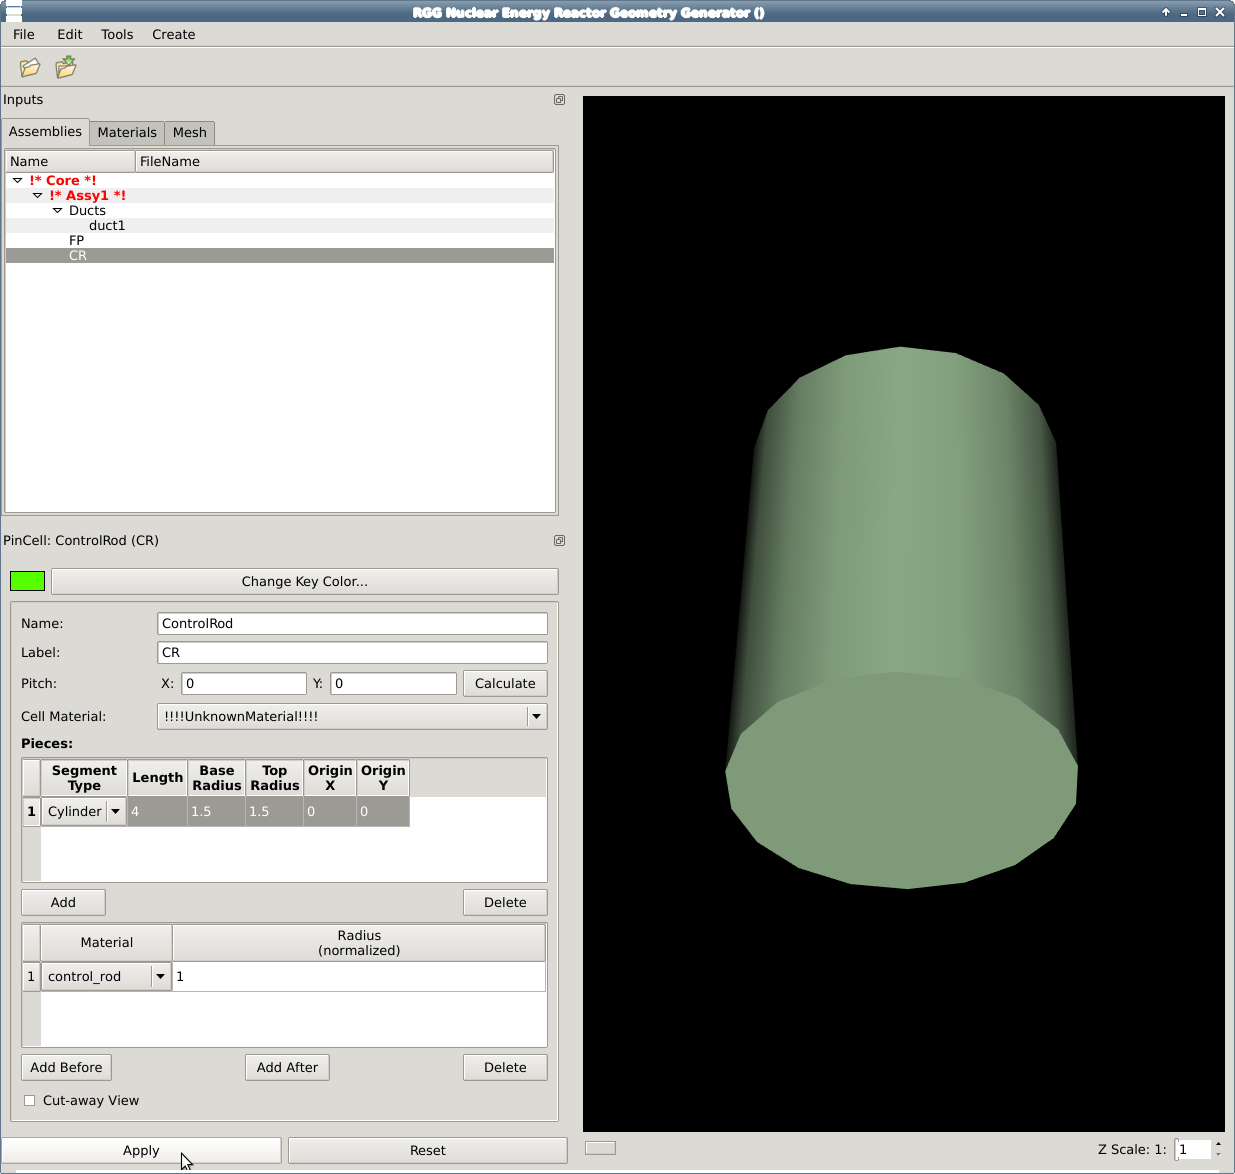
\includegraphics[width=0.48\textwidth]{Images/rect-7.png}
  \end{center}
  \caption{Final control product.}
  \label{fig:Rect7}
\end{wrapfigure}
Control rods are used to control nuclear fission. They are made out of materials which can easily absorb neutrons without undergoing fission themselves such as certain isotopes of boron, silver, or cadmium.

This is created using largely the same process as creating the fuel pin.  You can use the ``control rod'' material.  Once again, it's beneficial to change the key color to green.

Refer to ~\ref{fig:Rect7} for the final product.
\clearpage
\subsection{Adding Fuel Pins to the Assembly}

Now we want to add the pins we've created back to the assembly.  Click back on ``Assy 1'' in the assemblies view in order to see the assembly layout.  You should once again be able to see the water duct you created, and it should still be empty.  Compare your view with ~\ref{fig:Rect8}.

\begin{figure}[htb]
\begin{center}
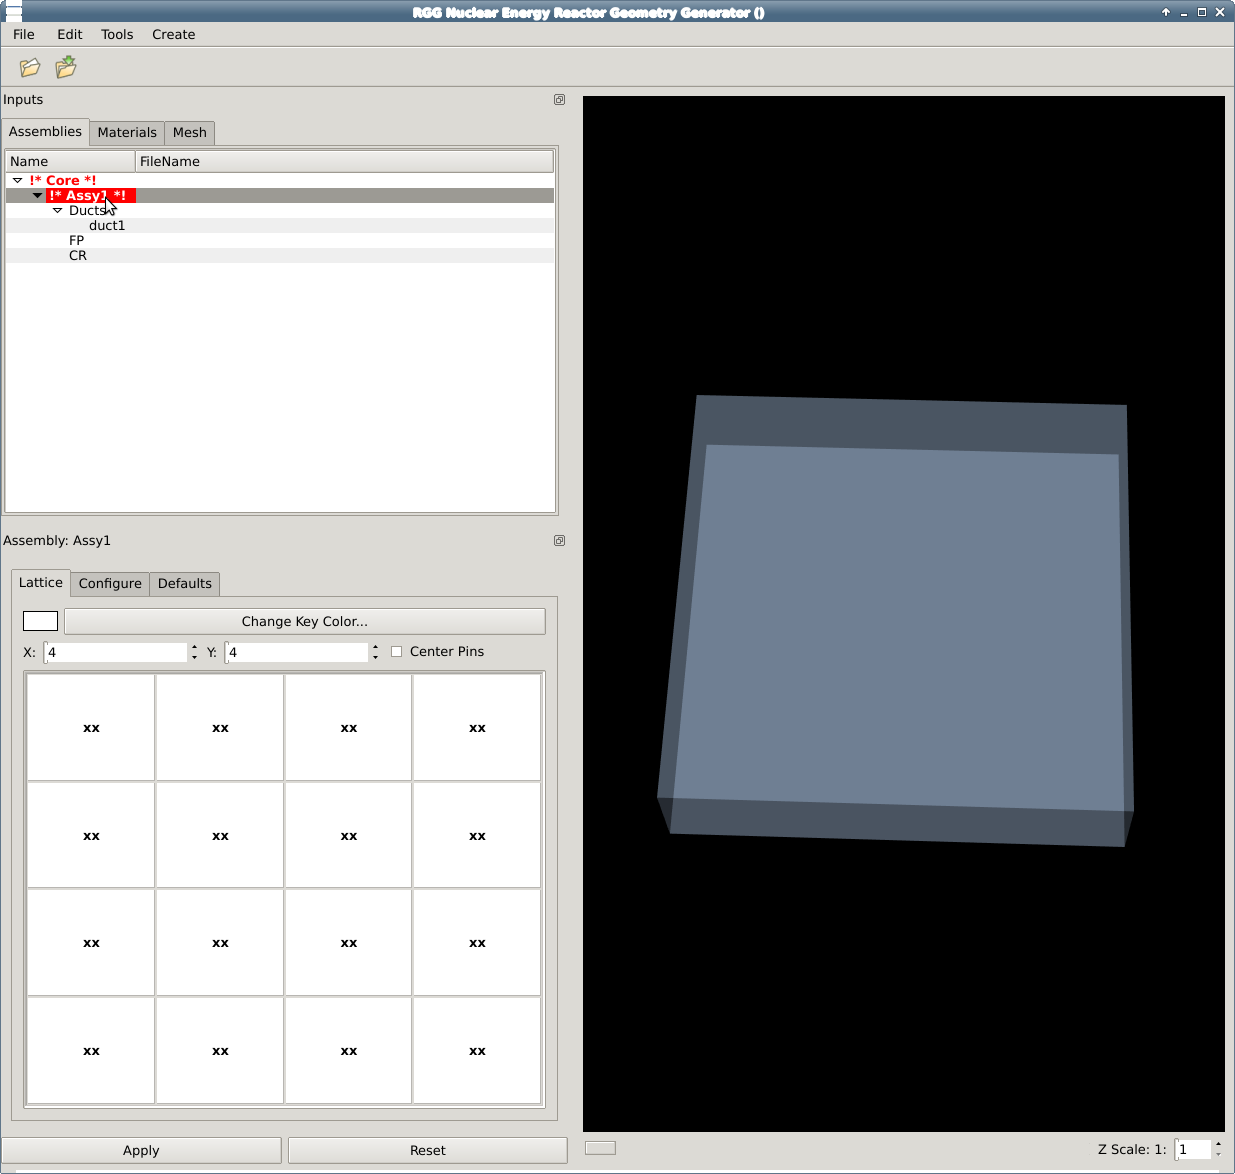
\includegraphics[width=0.4\linewidth]{Images/rect-8.png}
\caption{Empty duct in the assemblies view.}
\label{fig:Rect8}
\end{center}
\end{figure}

\begin{figure}[htb]
\begin{center}
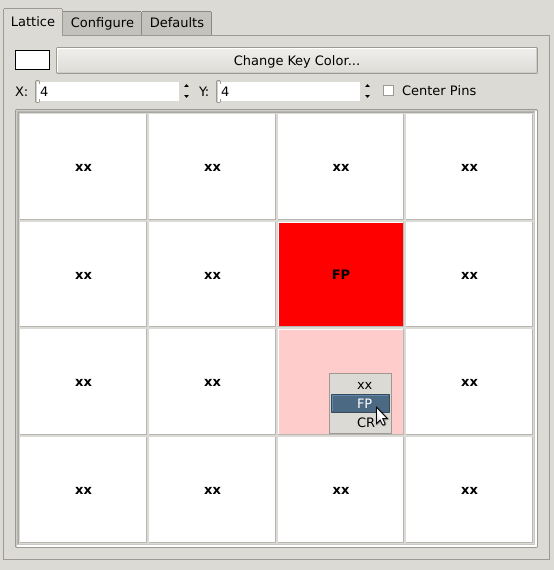
\includegraphics[width=0.4\linewidth]{Images/rect-9e1.png}
\caption{Right-click to organize the assembly.}
\label{fig:Rect9}
\end{center}
\end{figure}
Right click on each square and choose which pin to assign to it.  Alternatively, you can drag and drop pins already placed onto new squares.

In the end you should end up with something like ~\ref{fig:Rect10}.  If you find that the pins are placed in positions you didn't specify, go back to the pins and verify that the ``Pitch'' parameters are set to $X=4$ and $Y=4$ for each fuel pin and control rod.

Remember to click ``Apply'' in order to see your changes in the render window, or save them before navigating to another tab or pin.

\begin{figure}[htb]
\begin{center}
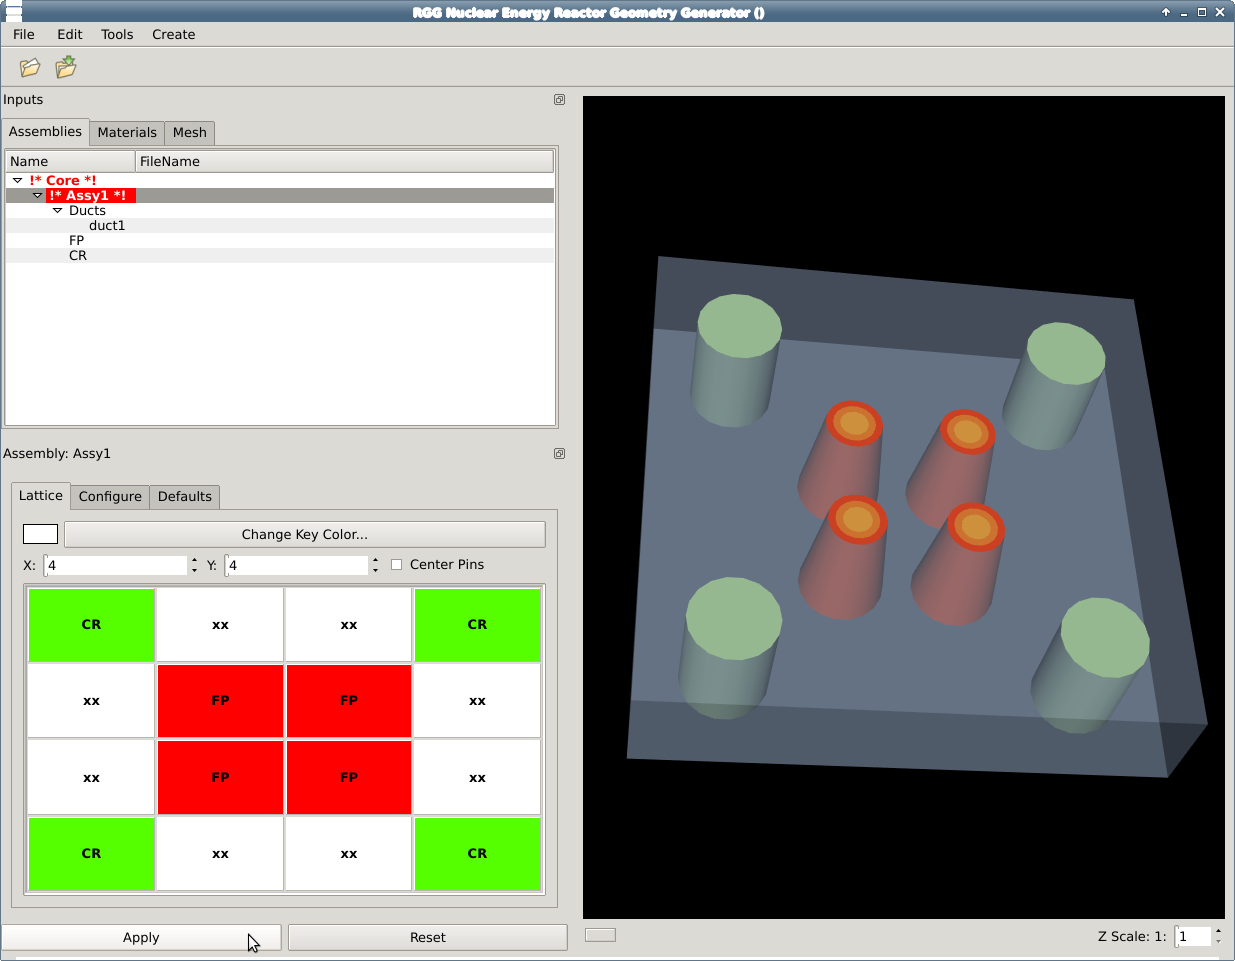
\includegraphics[width=0.7\linewidth]{Images/rect-10.png}
\caption{Final assembly.}
\label{fig:Rect10}
\end{center}
\end{figure}



\chapter{Example -- Building a Hexagonal Core}
\label{chapter:Example -- Building a Hexagonal Core}
\section{Make a new Hexagonal Core}

First, we'll need to create a new hexagonal core.

\begin{figure}[H]
	\begin{center}
		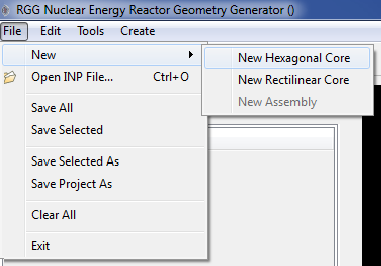
\includegraphics[width=0.5\linewidth]{Images/hex-1.png}
		\caption{Select the option to create a new hexagonal core.}
		\label{fig:Hex1}
	\end{center}
\end{figure}

The two panels on the left of the application will change.  We'll now see that the inputs panel contains an item named ``Core" with a subitem ``Assy1."  The core panel should show a hexagon labeled ``Assy1." Confirm that your application looks similar to what's shown in ~\ref{fig:Hex2}.

\begin{figure}[H]
	\begin{center}
		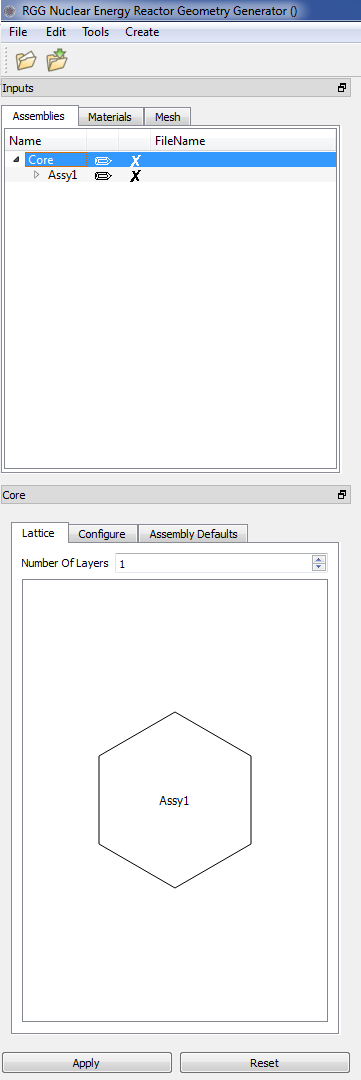
\includegraphics[width=0.2\linewidth]{Images/hex-2.png}
		\caption{The inputs and core panels after creating a new hexagonal core.}
		\label{fig:Hex2}
	\end{center}
\end{figure}

Next, we'll specify how many layers we'd like our lattice to have.  In the core panel, either type in the number of desired layers or use the buttons to the right of the field to increment and decrement the number.  The panel should look something like what's displayed in ~\ref{fig:Hex3}.

\begin{figure}[H]
	\begin{center}
		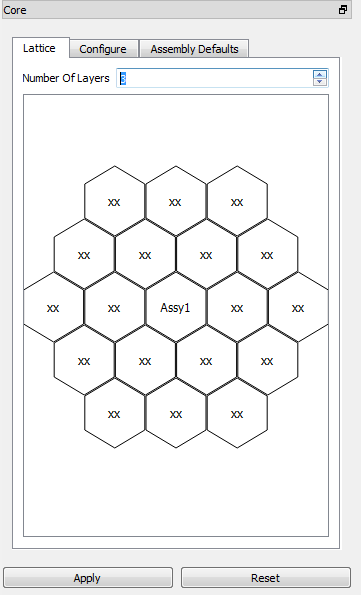
\includegraphics[width=0.5\linewidth]{Images/hex-3.png}
		\caption{Updating the number of layers of the core.}
		\label{fig:Hex3}
	\end{center}
\end{figure}

Be sure to click the apply button below to see apply changes.

\begin{figure}[H]
	\begin{center}
		
\includegraphics[width=0.5\linewidth]{Images/hex-4.png}
		\caption{The apply button.}
		\label{fig:Hex4}
	\end{center}
\end{figure}

\section{Configuring the Assembly}
\label{section:RotateAssembly30}
We need to configure the hexagonal ducts and pins we'll create to be rotated by 30 degrees to avoid interference from the different cells.  To do this, first ensure that you're clicking on the assembly we created, as shown in ~\ref{fig:Hex15}.

\begin{figure}[H]
	\begin{center}
		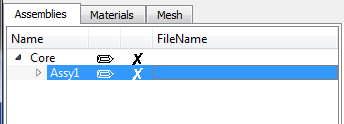
\includegraphics[width=0.5\linewidth]{Images/hex-15.png}
		\caption{Clicking on our assembly.}
		\label{fig:Hex15}
	\end{center}
\end{figure}

Then, we need to click on the configure tab in the lower panel, and scroll down to the section labeled transform.  Click the Add Rotation button.

\begin{figure}[H]
	\begin{center}
		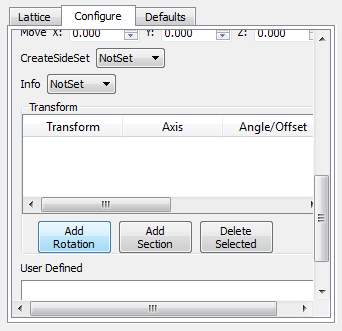
\includegraphics[width=0.5\linewidth]{Images/hex-16.png}
		\caption{Assembly transformations.}
		\label{fig:Hex16}
	\end{center}
\end{figure}

We need to change this rotation to be 30 degrees.  Enter 30 as shown in ~\ref{fig:Hex17}.

\begin{figure}[H]
	\begin{center}
		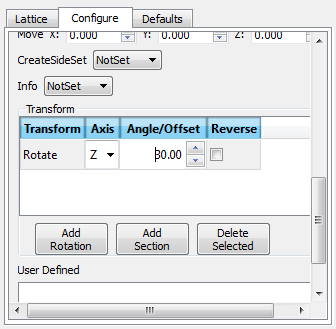
\includegraphics[width=0.5\linewidth]{Images/hex-17.png}
		\caption{Adding the 30 degree transformation.}
		\label{fig:Hex17}
	\end{center}
\end{figure}

As always, please click Apply to make sure that your changes are saved.

\section{Adding a duct to the Assembly}

\subsection{Creating the Duct}

Now that we have set up our core and configured the assembly, we need to create a duct.  To do this, follow ~\ref{fig:Hex5}.

\begin{figure}[H]
	\begin{center}
		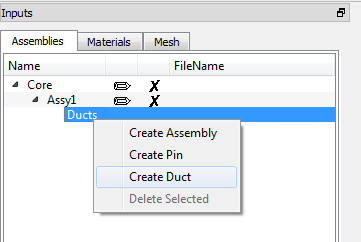
\includegraphics[width=0.5\linewidth]{Images/hex-5.png}
		\caption{Creating a duct.}
		\label{fig:Hex5}
	\end{center}
\end{figure}

Your screen should now look like this:

\begin{figure}[H]
	\begin{center}
		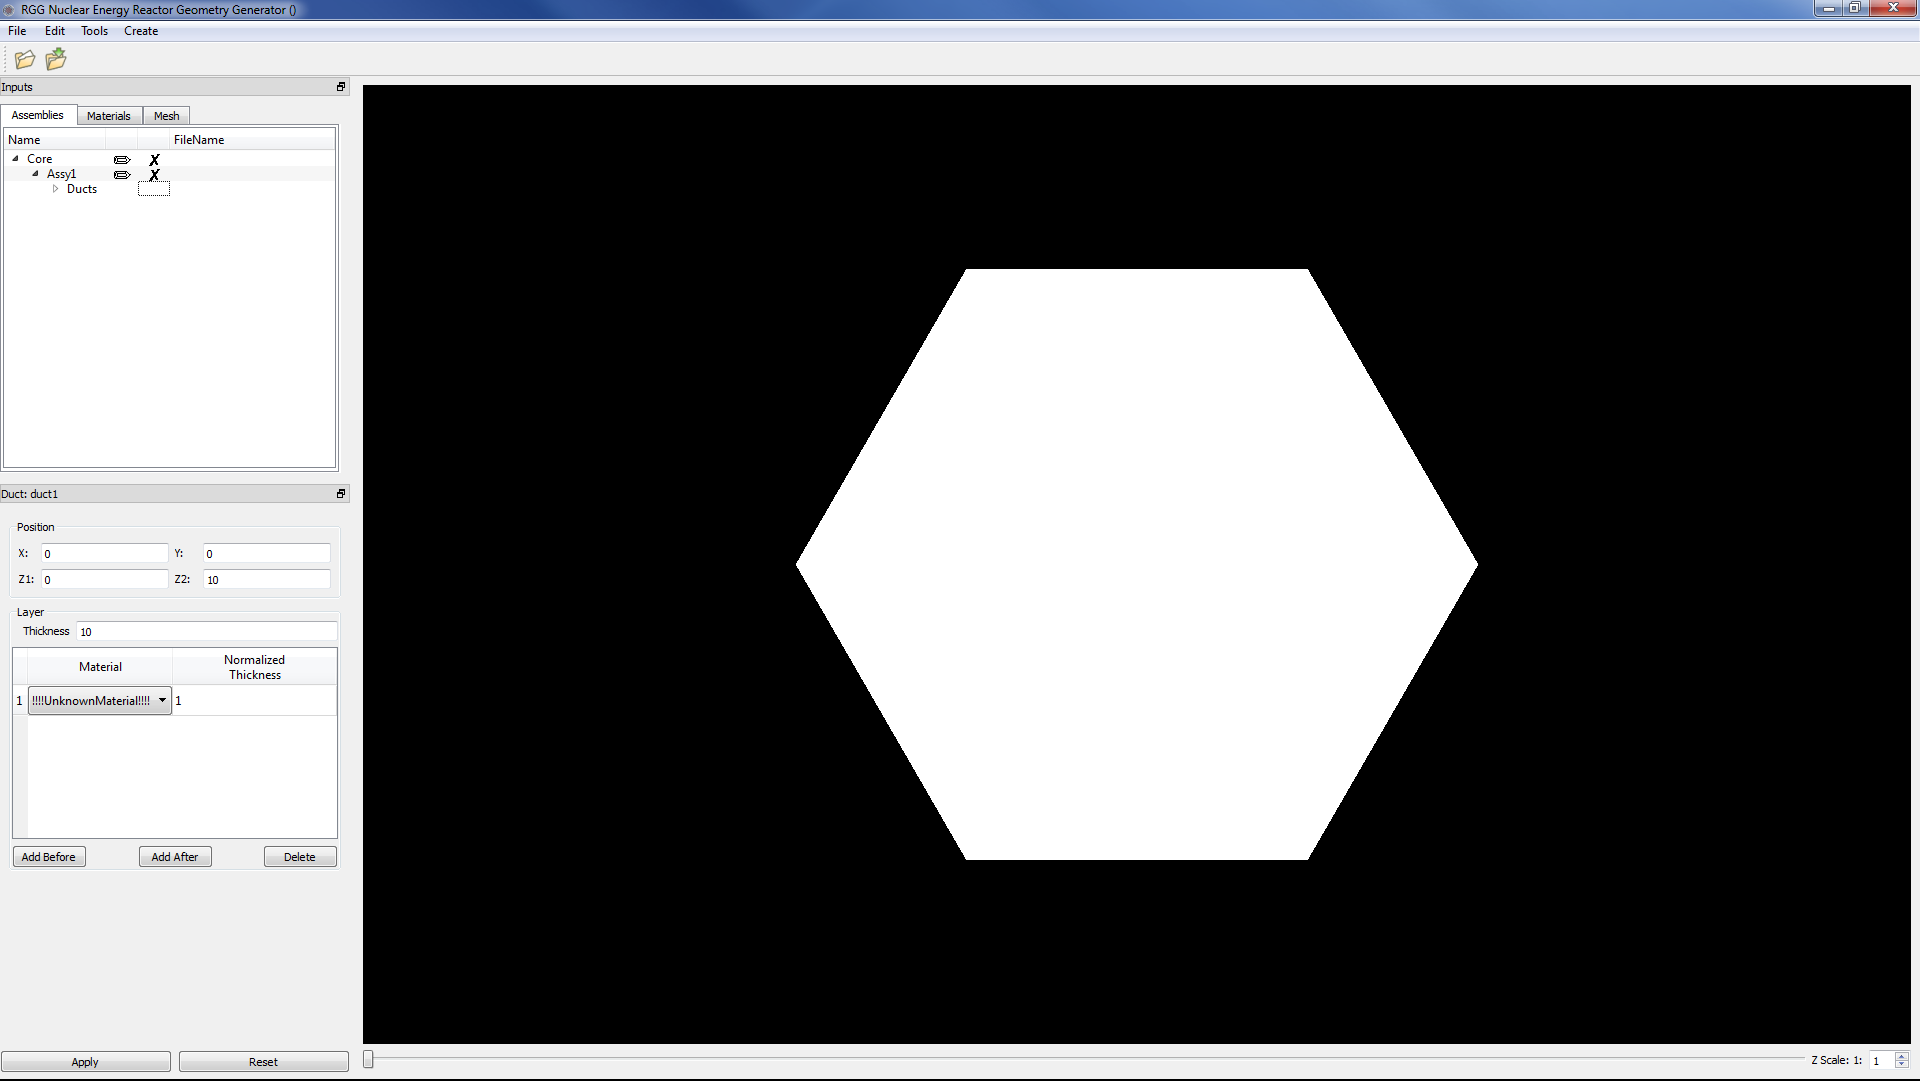
\includegraphics[width=0.85\linewidth]{Images/hex-6.png}
		\caption{Your screen after adding duct.}
		\label{fig:Hex6}
	\end{center}
\end{figure}

\subsection{Configuring Duct}

We now need to configure the duct we created.  In the inputs panel, select the duct.  This will change the lower panel to show the materials of the duct and the normalized radii of those materials.  For this duct, we'll stay simple and make the material water.  Change the material type to water by clicking the drop-down and selecting ``water."

\begin{figure}[H]
	\begin{center}
		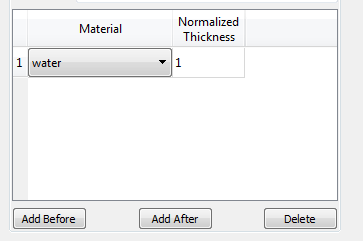
\includegraphics[width=0.5\linewidth]{Images/hex-7.png}
		\caption{Selecting water as our material.}
		\label{fig:Hex7}
	\end{center}
\end{figure}

Your screen should now look like ~\ref{fig:Hex8}.

\begin{figure}[H]
	\begin{center}
		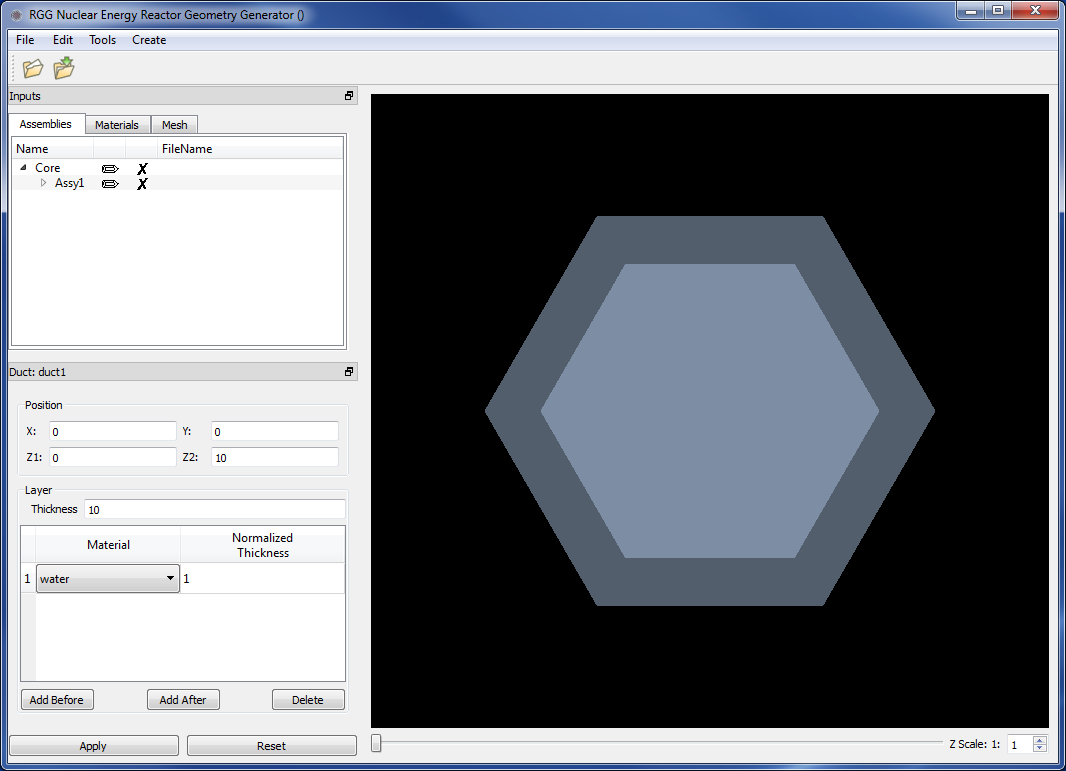
\includegraphics[width=0.5\linewidth]{Images/hex-8.png}
		\caption{Creating a duct.}
		\label{fig:Hex8}
	\end{center}
\end{figure}

\section{Adding a Pin}
\subsection{Creating a Pin}

To create a pin in the assembly, right click on the name of the assembly and select ``Create Pin."

\begin{figure}[H]
	\begin{center}
		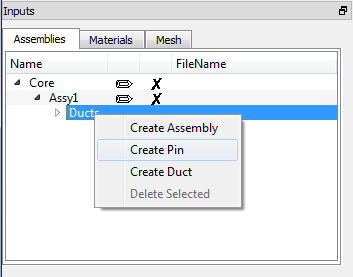
\includegraphics[width=0.5\linewidth]{Images/hex-9.png}
		\caption{Creating a pin.}
		\label{fig:Hex9}
	\end{center}
\end{figure}

\subsection{Configuring the Pin}

You can edit the name, label, pitch, and cell material of the pin.  Refer to ~\ref{fig:Hex10} to see how to change them.  We will leave them to the defaults.

\begin{figure}[H]
	\begin{center}
		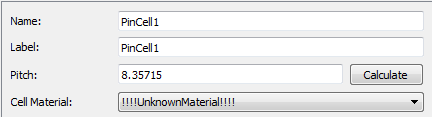
\includegraphics[width=0.5\linewidth]{Images/hex-10.png}
		\caption{Name, label, pitch, and cell material for a pin.}
		\label{fig:Hex10}
	\end{center}
\end{figure}

We now need to add pieces of the pin.  There are two kinds of pin pieces: frustrums and cylinders.  We'll add a cylinder by clicking the add button.

\begin{figure}[H]
	\begin{center}
		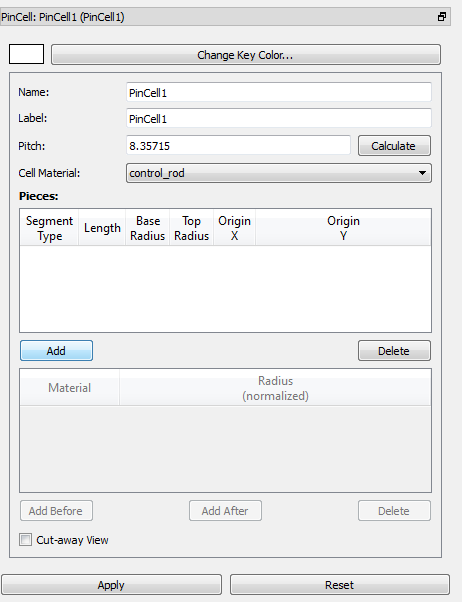
\includegraphics[width=0.5\linewidth]{Images/hex-11.png}
		\caption{Adding a pin piece.}
		\label{fig:Hex11}
	\end{center}
\end{figure}

Then, confirm that our segment type is a cylinder, and that the sum of the length of the segments is equal to the length of the duct (10).

\begin{figure}[H]
	\begin{center}
		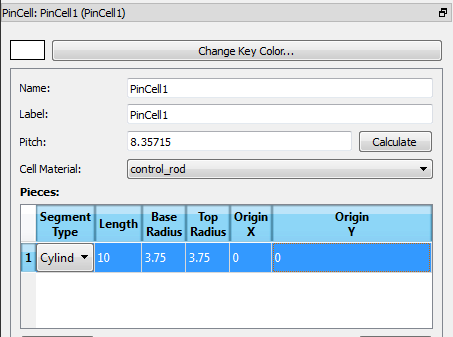
\includegraphics[width=0.5\linewidth]{Images/hex-12.png}
		\caption{Confirming our cylinder's configuration.}
		\label{fig:Hex12}
	\end{center}
\end{figure}

Now, we're going to modify the material of this cylinder.  We'll make this a control rod, so we'll change the material to match.

\begin{figure}[H]
	\begin{center}
		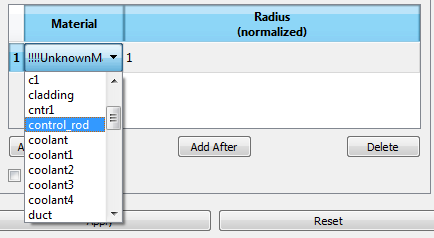
\includegraphics[width=0.5\linewidth]{Images/hex-13.png}
		\caption{Changing the material to be a control rod.}
		\label{fig:Hex13}
	\end{center}
\end{figure}

Be sure to press apply to ensure your changes go into effect.

We should see a screen like the after we're done:

\begin{figure}[H]
	\begin{center}
		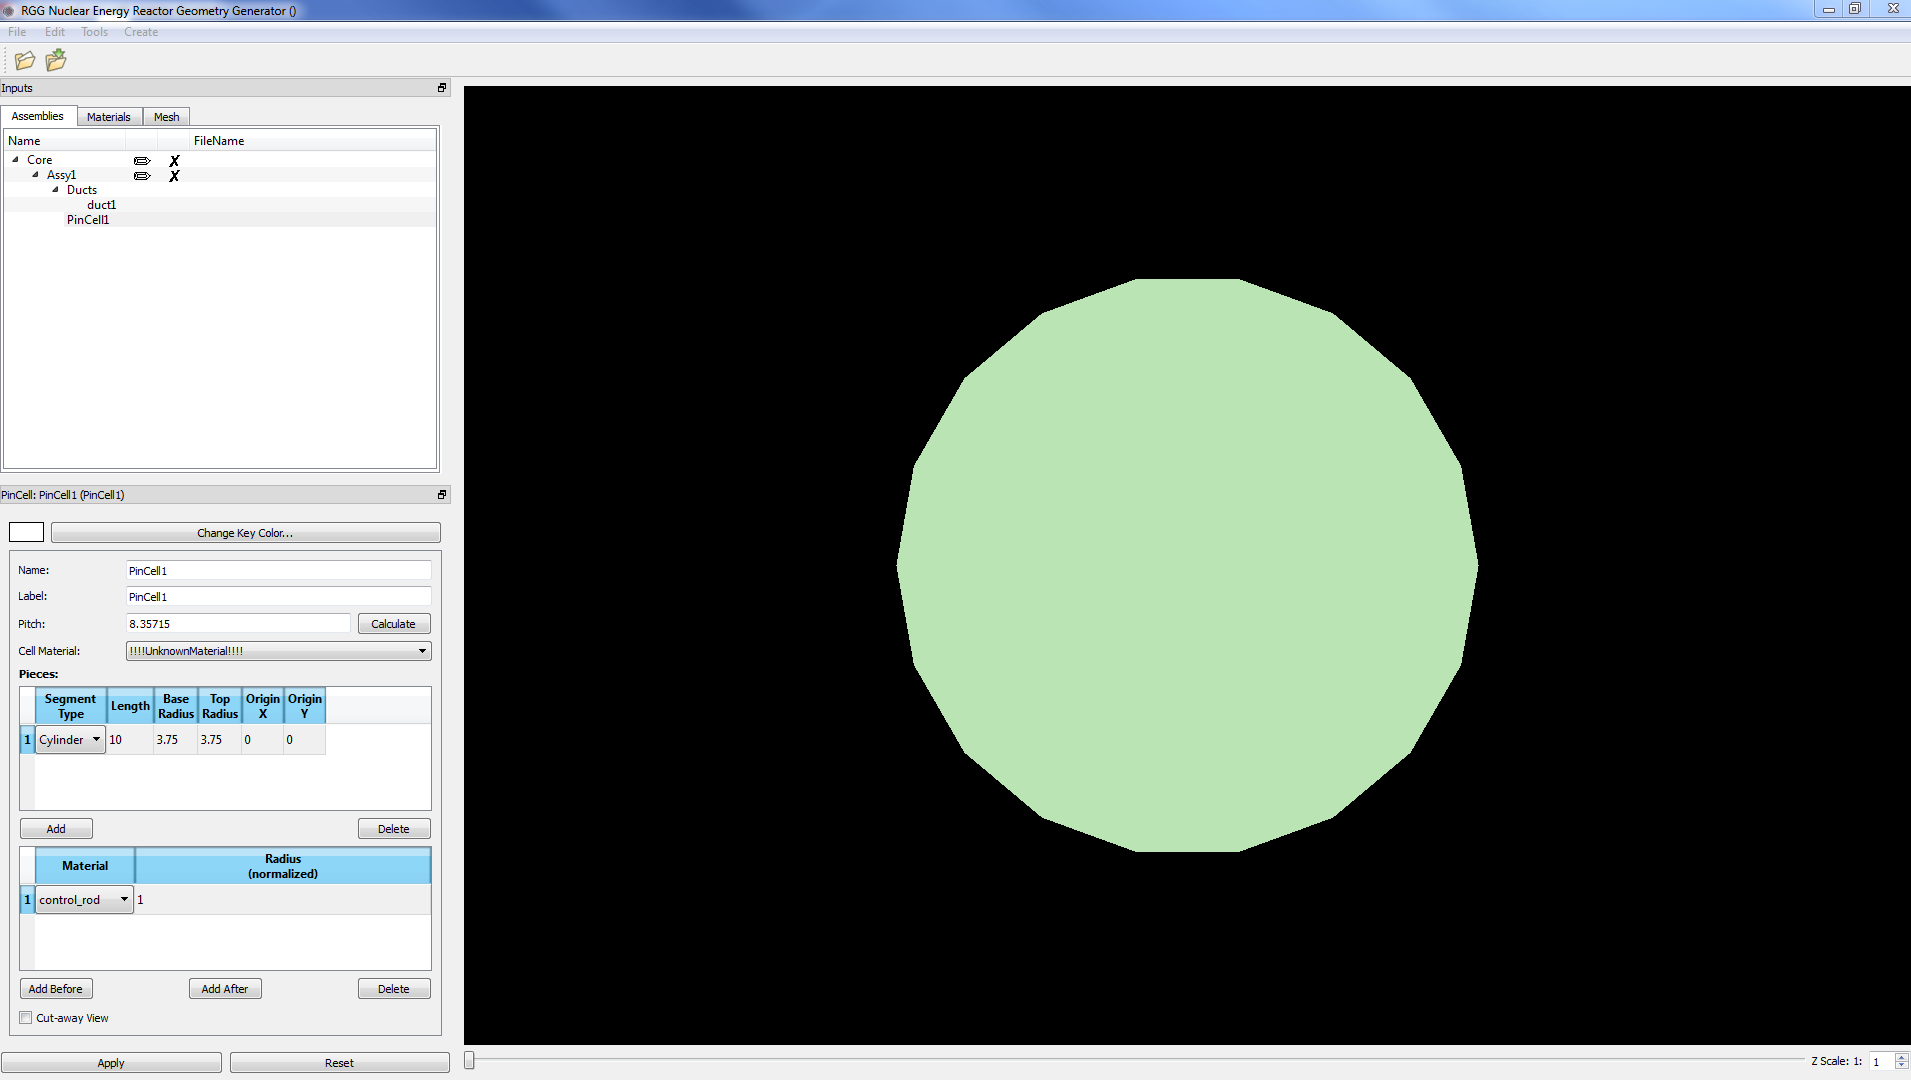
\includegraphics[width=0.85\linewidth]{Images/hex-14.png}
		\caption{After adding the cylinder.}
		\label{fig:Hex14}
	\end{center}
\end{figure}

Next, we need to add this pin to our assembly lattice.  Make sure you select ``Assy1" in the inputs menu.  Click the lattice tab in the lower panel, and right click on the hexagon to bring up a list of available pins.  Select our pin.

\begin{figure}[H]
	\begin{center}
		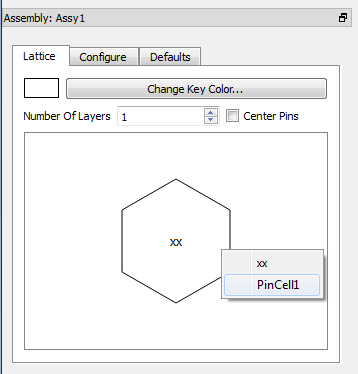
\includegraphics[width=0.5\linewidth]{Images/hex-18.png}
		\caption{Selecting our pin for the assembly.}
		\label{fig:Hex18}
	\end{center}
\end{figure}

Click the apply button to save your changes.

\section{Populating core with our assembly}

Click on our assembly (``Assy1") in the inputs pane.  In the lower pane, click on the lattice tab.  To add the assembly to any of the cells, right click to bring up a list of available assemblies, and then click on the assembly you'd like.

\begin{figure}[H]
	\begin{center}
		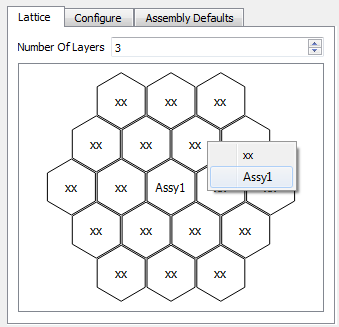
\includegraphics[width=0.5\linewidth]{Images/hex-19.png}
		\caption{Selecting assembly for a cell.}
		\label{fig:Hex19}
	\end{center}
\end{figure}

We'll select Assy1 because that's the name of the assembly we'd like.  Make sure to click the apply button to make sure that the changes we've made are applied.  Your screen should look like the following when you're done.

\begin{figure}[H]
	\begin{center}
		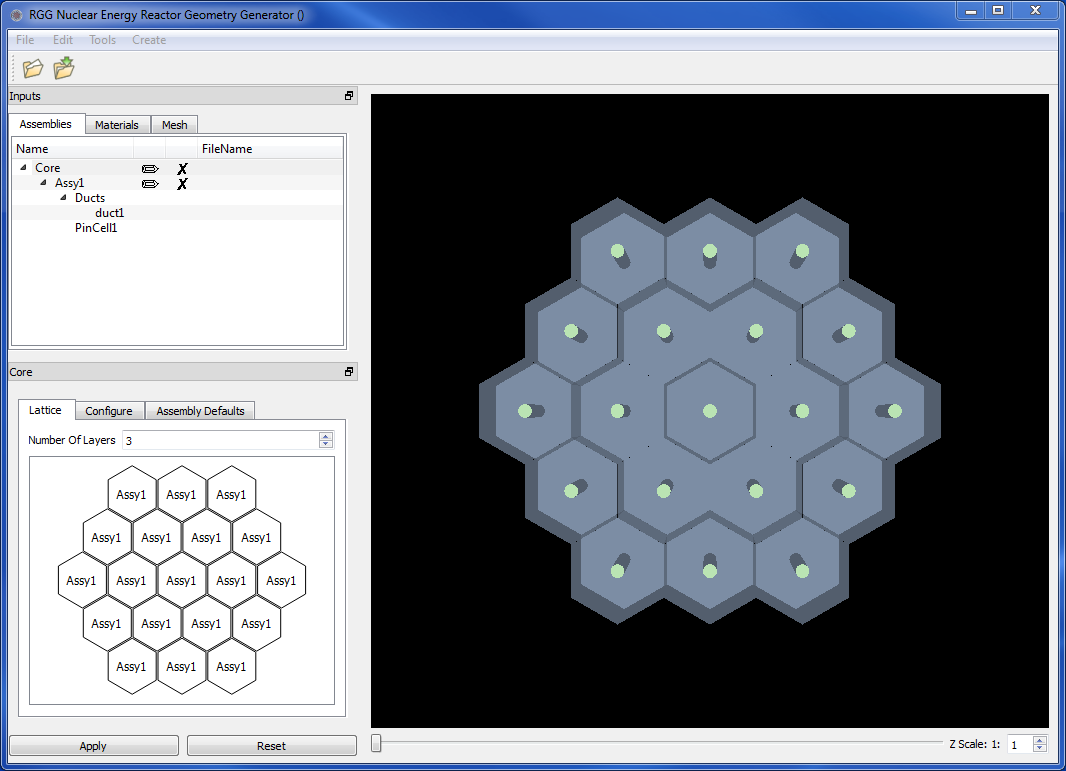
\includegraphics[width=0.85\linewidth]{Images/hex-20.png}
		\caption{Final view.}
		\label{fig:Hex20}
	\end{center}
\end{figure}

Congratulations!  You've made a hexagonal core!

\chapter{Specifying Meshing Control Information}
\label{chapter:Specifying Meshing Control Information}
 Vivamus et dolor ut mi dignissim dictum non at nulla. Donec a enim ut turpis aliquet gravida. Morbi consectetur porta tellus eu facilisis. Aliquam sed nisi viverra, mattis dui eget, ultrices ipsum. Praesent imperdiet hendrerit eros, ut iaculis est aliquam ut. Ut quis orci rutrum, gravida risus id, vulputate sem. Aliquam rutrum purus velit, ac aliquam massa egestas ut. Duis euismod vestibulum volutpat. Phasellus aliquet nulla in nisi consectetur, quis convallis arcu ultrices. Phasellus et tellus dui. Praesent nisl ligula, accumsan auctor ornare sit amet, vulputate auctor risus. Duis tellus risus, adipiscing at tristique nec, volutpat ac nisi. Sed sodales augue ac nunc ornare consectetur. Etiam consectetur aliquet erat, sed interdum lorem iaculis et. Donec eleifend pretium diam, non pretium quam. Nullam molestie enim in nunc hendrerit aliquam.

\chapter{Interfacing with MeshKit Tools and Cubit}
\label{chapter:Interfacing with MeshKit Tools and Cubit}
Nunc viverra varius odio, at pharetra velit laoreet nec. Donec sagittis vestibulum erat posuere auctor. Ut at interdum tortor, volutpat ullamcorper massa. Vestibulum a tempus quam, sed fringilla nibh. Nam semper est a ante venenatis, non bibendum lectus auctor. Duis blandit lacus urna, eget dictum sem pretium eget. Etiam bibendum semper placerat. Pellentesque commodo eros tempor justo congue, vel aliquam quam tristique. Donec eu magna ornare nisl vulputate pretium. Pellentesque at orci et velit luctus elementum eu eget dui. In hac habitasse platea dictumst.

\chapter{Displaying Meshes}
\label{chapter:Displaying Meshes}
\section{Displaying the Mesh}
\label{section:DisplayingMeshes}

Upon successful creation of a mesh, you either need to load it in manually via the \emph{open MOAB file dialog} accessed from the \emph{open MOAB file item} in the \emph{file menu}, or, if you've just meshed an INP file you lodaed in, the mesh will load in automatically.

\subsection{Views of the Mesh}
To control viewing the mesh, be sure to click on the \emph{mesh tab} of the \emph{inputs panel}.  RGG allows you to six different options to control the \emph{3D view} of the mesh, listed below:

\begin{itemize}
	\item{Volumes}
	\item{Boundary}
	\item{Surfaces}
	\item{Neumann Sets}
	\item{Dirichlet Sets}
	\item{Material Sets}
\end{itemize}

More detail on these views is provided below.  Additionally, you can check the \emph{show edges checkbox} to view the mesh superimposed on the 3D view and check the \emph{color checkbox} to colorize the different pieces of the view based on the option you've selected.

\subsubsection{Volumes}
Clicking the \emph{volumes option} shows all the volumes of the mesh.  Checking the color checkbox will colorize all of the distinct volumes in different colors.

\subsubsection{Boundary}
In this mode, RGG displays only the boundary conditions.  Checking the color checkbox will colorize all of the distinct volumes in different colors.

\subsubsection{Surfaces}
When the \emph{surfaces option} is selected, RGG displays only the surfaces of the mesh.

\subsubsection{Neumann Sets}
Clicking the \emph{Neumann Sets option} will show the natural boundary conditions on sides of domains.

\subsubsection{Dirichlet Sets}
Clicking the \emph{Dirichlet Sets option} will show the essential boundary conditions on points of domains.

\subsubsection{Material Sets}
Material sets displays all the volumes of the mesh, but colorizes them on a per material basis.  Additionally, you can toggle the visability of materials by checking and unchecking them in the \emph{materials tab} of the inputs panel.

\end{document}
